\chapter{OpenFOAM PDE and RDE Modeling}
\label{solvtestchap}

\section{Preface}

This chapter will go through progression of research on efficacy for the different solvers and PDE/RDE modeling techniques performed during the duration of this thesis work. In an effort to assist the University of Colorado's Turbulence and Energy Systems Laboratory (TESLa), several solvers and methods will be tested for potential for detonation modeling, stability, and accuracy, typically in that order. 

\section{Modeling Progression}
\subsection{Initial Attempts}
To begin on the problem of modeling detonations in OpenFOAM, the included tutorials folder as well as the geometric and initial condition setup of located in a related TESLa paper by Towery\cite{towery1} was utilized to begin the work towards an OpenFOAM model of a linear detonation tube/PDE.

Firstly, the detonation of methane fuel and oxygen oxidizer without inert nitrogen filler was explored within a 2D detonation tube with the solver \verb|rhoReactingFoam|. A region of high temperature methane and oxygen on the left hand side was used to initiate the detonation. In the PDE and detonation simulations presented in this paper, stoichiometric fuel and oxidizer was premixed and available thoughout the domain. Solid walls on the left, top, and bottom of the tube were used. The exit was set as a special \verb|waveTransmissive| boundary condition that allows for shockwaves to not reflect at the exit and for gases to expel as well. A detonation was successfully created with this, but the accuracy and stability were still untested. In order to check that the boundary conditions being applied were correct, a small detonation cell of high pressure and temperature was set in the bottom left corner of the tube. As the simulation progressed, correct wave reflection was seen on the sides of the tube as well as some wave transmissive behavior from the exit was seen (Figure \ref{fig:cornerdet}). 
\begin{figure}[b]
\centering
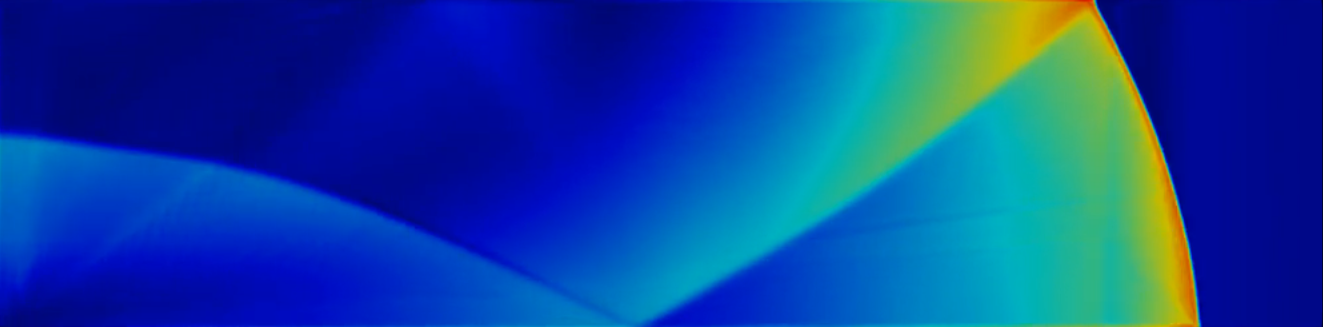
\includegraphics[width=\linewidth]{figs/cornerdet.png}
\caption{Initial methane and oxygen detonation boundary condition test with corner detonation. Velocity magnitude is plotted here without scale to just check the solver and boundary conditions for modeling potential. Detonation was initiated in the lower left corner.}
\label{fig:cornerdet}
\end{figure}%
\noindent It was noticed that the exit boundary condition was expelling gas in a rectangular region long before the detonation wave(s) reached the exit, so some tweaking was done on this \verb|waveTransmissive| boundary condition in order to make it more accurate. The boundary condition option accepts inputs such as ratio of specific heats, expected flow velocity, far-field conditions and distance from exit plane, and names of some variables such as the condition to track at the exit as well as some flux variables. 

The next step with \verb|rhoReactingFoam| was to start progressing towards testable detonation results. To do this, a change from methane to hydrogen for the fuel was selected. This fuel change was done to better match papers such as those being produced by TESLa as well as the general experimental and computational detonation modeling community. The exact geometric detontion tube was taken from Towery\cite{towery1} for comparison as well as the initial detonation size and thermodynamic conditions. Additionally, inert nitrogen was added into the tube to transition from hydrogen-oxygen to hydrogen-air. In accordance with trying to double check whether results made sense with Towery\cite{towery1}, the Arrhenius rate equation was used for reaction rates. An issue that was problematic starting this research was that the documentation for the units within the \verb|reactions| file were conflicting. Much testing was performed at this stage in an attempt to determine the units that OpenFOAM uses for the reactions given in this file, especially regarding the pre-exponential factor. While some ground was gained on this, a shift of focus towards the solver performed in order to determine if \verb|rhoReactingFoam| was appropriate for capturing shocks. 

The Sod shock tube problem was utilized to determine if the OpenFOAM solvers used were capturing shocks accurately. 






